\documentclass[12pt]{article}
\usepackage{setspace, amsmath, mathdots, amssymb, graphicx, multirow, gensymb, slashbox, listings, enumerate}
\usepackage[margin=1.5in]{geometry}
\onehalfspacing

\begin{document}

\noindent STA 250 HOMEWORK 4 \newline Yichuan Wang \newline \newline
Problem 1 \newline \newline
In the first problem of this homework, I implemented the method proposed by Robert (2009) in CUDA code in order to obtain samples from a truncated normal distribution with given parameters. The distribution can be represented as
\begin{center}
	$TN(\mu, \sigma^2; a, b)$
\end{center}
where $\mu$ and $\sigma^2$ are the mean and variance of the original, i.e. untruncated, normal distribution and $a, b$ represent the lower and upper bounds of the truncation interval with $a \geq -\infty, b \leq \infty$. Provided in the lecture notes, the expected values for a random variable $Z \sim TN(\mu, \sigma^2; a, b)$ is
\begin{center}
$E(Z) = \begin{cases}
	\mu - \sigma \frac{\phi(\frac{b-\mu}{\sigma})}{\Phi(\frac{b-\mu}{\sigma})} &\mbox{if }a = -\infty, b < \infty \\
	\mu + \sigma \frac{\phi(\frac{a-\mu}{\sigma})}{1-\Phi(\frac{a-\mu}{\sigma})} &\mbox{if }a > -\infty, b = \infty \\
	\mu + \sigma \frac{\phi(\frac{a-\mu}{\sigma})-\phi(\frac{b-\mu}{\sigma})}{\Phi(\frac{b-\mu}{\sigma})-\Phi(\frac{a-\mu}{\sigma})} &\mbox{if }a > -\infty, b < \infty
\end{cases}$
\end{center}
where $\phi, \Phi$ are p.d.f and c.d.f of the standard normal distribution respectively. \newline
As directed in the paper by Robert (2009), when the truncation region is one-sided, for example $TN(0, 1;\mu^-, \infty)$, the algorithm for sampling from such truncated normal goes as follows:
\begin{enumerate}[(1)]
	\item Generate a random sample $z = \mu^- + Expo(\alpha)$, where $Expo(\alpha)$ stands for a random number generated from the exponential distribution with parameter $\alpha$.
	\item Compute the value $\psi(z)$ where \newline
		$\psi(z) = \begin{cases} \exp(-\frac{(\alpha - z)^2}{2}) &\mbox{if } \mu^- < \alpha \\ \exp(-\frac{(\mu^--\alpha)^2}{2})\exp(\frac{(\alpha-z)^2}{2}) &\mbox{if } \mu^- \geq \alpha \end{cases}$.
	\item Sample $u$ from $U[0,1]$, if $u < \psi(z)$ then we accept $z$ as our sample for this iteration; otherwise go back to step (1).
\end{enumerate}
When the truncation region is one-sided but with an upper truncation, for example $TN(0, 1;-\infty, \mu^+)$, we may simple reverse the sign of $\mu^+$ and sample from lower truncation case then reverse the sign back. Also the optimal choice of parameter $\alpha$ for the exponential distribution is $\alpha_* = \frac{\mu^-+\sqrt{(\mu^-)^2+4}}{2}$.\newline
When we have a two-sided truncation, e.g. $TN(0, 1,;\mu^-, \mu^+)$, the algorithm is:
\begin{enumerate}[(1)]
	\item Sample $z$ from $U[\mu^-, \mu^+]$.
	\item Compute $\psi(z) = \begin{cases}
		\exp(-\frac{z^2}{2}) &\mbox{if } 0 \in [\mu^-, \mu^+] \\
		\exp(-\frac{(\mu^-)^2 - z^2}{2}) &\mbox{if } \mu^- > 0\\
		\exp(-\frac{(\mu^+)^2 - z^2}{2}) &\mbox{if } \mu^+ < 0
	\end{cases}$
	\item Sample $u$ from $U[0,1]$, if $u < \psi(z)$, we accept z; otherwise, go back to step (1).
\end{enumerate}
For any truncated normal distribution where $\mu \neq 0$ and/or $\sigma \neq 1$, we may simple use location-scale transformation to obtain properly transformed truncation region then transform the samples back to corresponding ones in the desired distribution.\newline
After executing the code on AWS to generate 10000 samples from distribution $TN(2,1;0, 1.5)$, the expected value was calculated to be $0.957$, and the mean of samples were $0.849$. The two values are not very close but not too far away. It could be due to some coding error when implementing the algorithm from Robert (2009). \newline
Another trial was executed in R with the function rtnorm() from "msm" package to generate 10000 samples from the same truncated normal distribution. This time the mean of 10000 random samples turned out to be $0.954$, which is quite close to the expected value.\newline
Then both the CUDA and R code were put to test to generate $10^k$ samples, $k = 1, \cdots, 8$, still from the distribution $TN(2,1;0, 1.5)$. The mean values for samples generated by GPU and CPU are
\begin{center}
	\begin{tabular}{|c|c|c|c|c|c|c|c|c|}
	\hline
	$k=$ & 1 & 2 & 3 & 4 & 5 & 6 & 7 & 8 \\
	\hline
	GPU & 0.871 & 0.812 & 0.843 & 0.849 & 0.849 & 0.849 & 0.849 &  0.849 \\
	\hline
	CPU & 1.343 & 0.946 & 0.950 & 0.954 & 0.957 & 0.957 & 0.957 & 0.957 \\
	\hline
	\end{tabular}
\end{center}
Both CUDA and R codes returned "converged" mean values when sample size became large. However, the R code gave closer estimate of the expected value for the truncated normal distribution. \newline
When looking at the cost/time of completing the tasks, GPU showed significant gain over CPU in terms of requiring less time to complete tasks when the sample size is large. The following are three figures, each for "User Time", "System Time" and "Elapsed Time":\newline
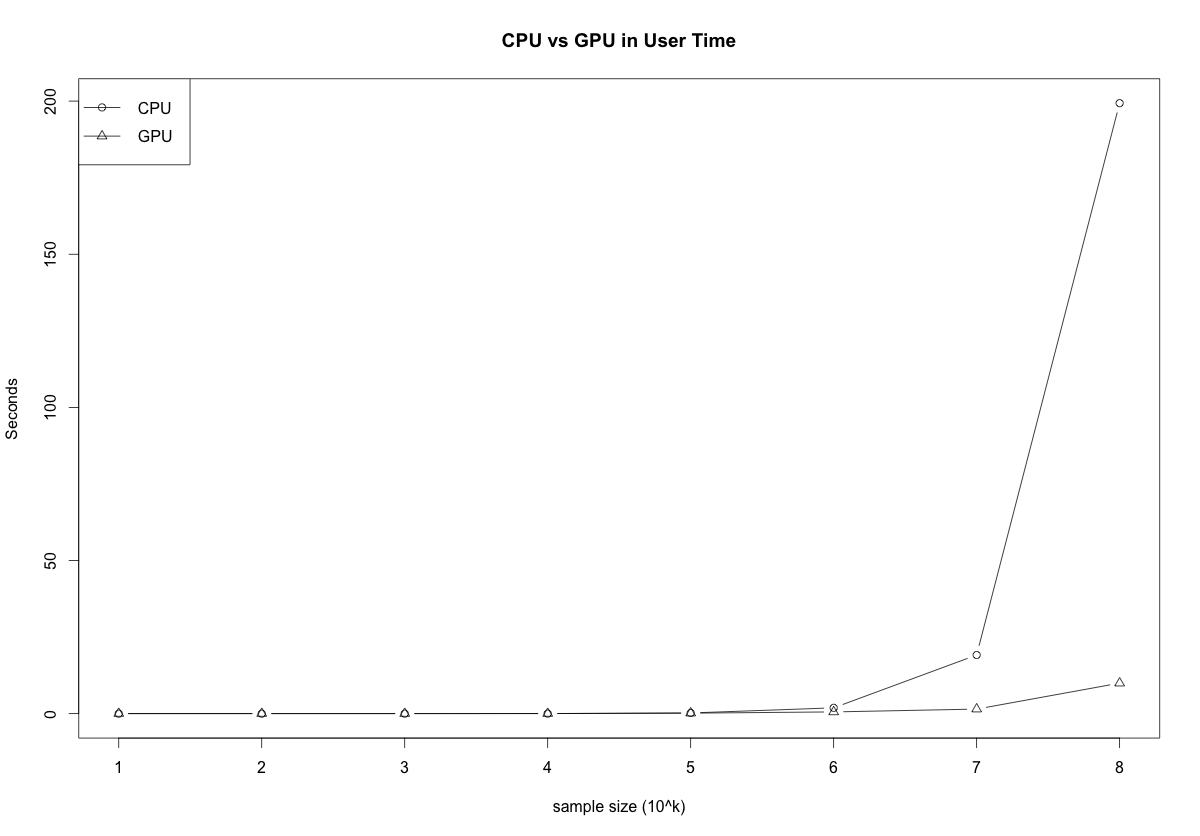
\includegraphics[width=\textwidth]{cpuvsgpuut.png}\newline
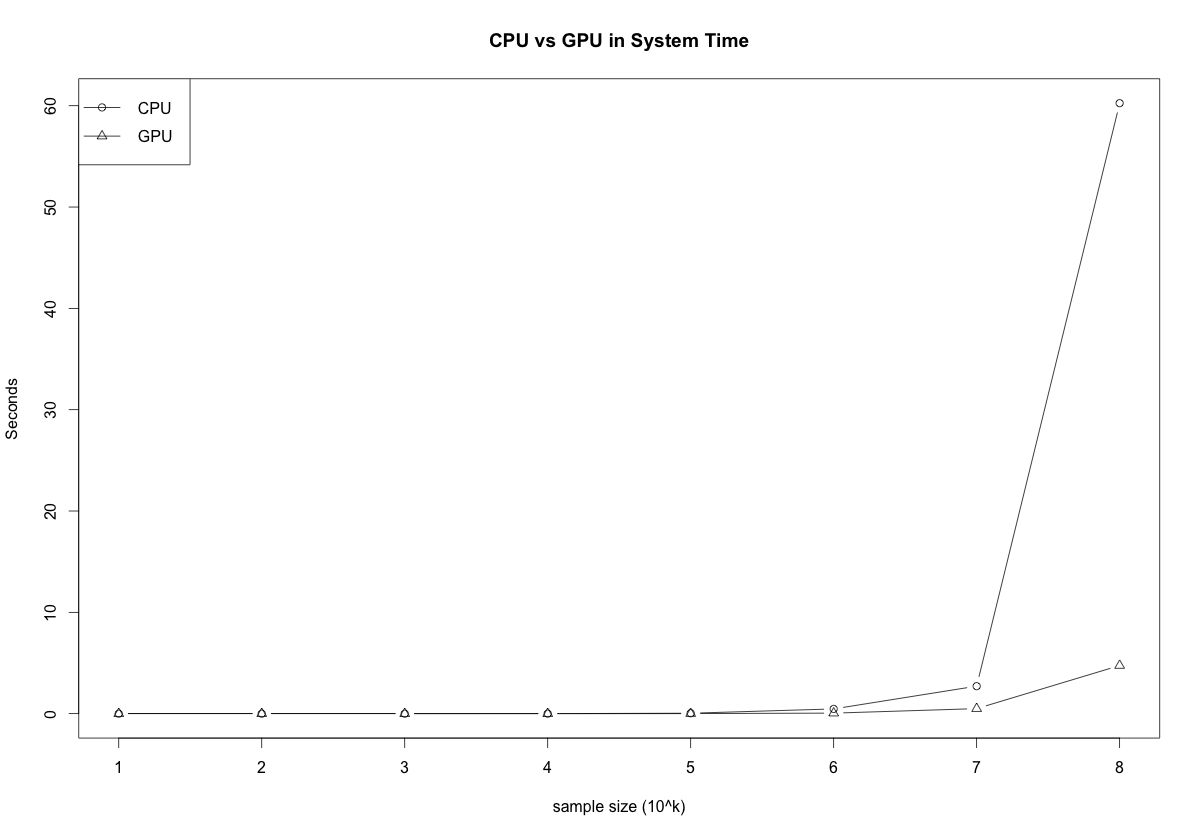
\includegraphics[width=\textwidth]{cpuvsgpust.png}\newline
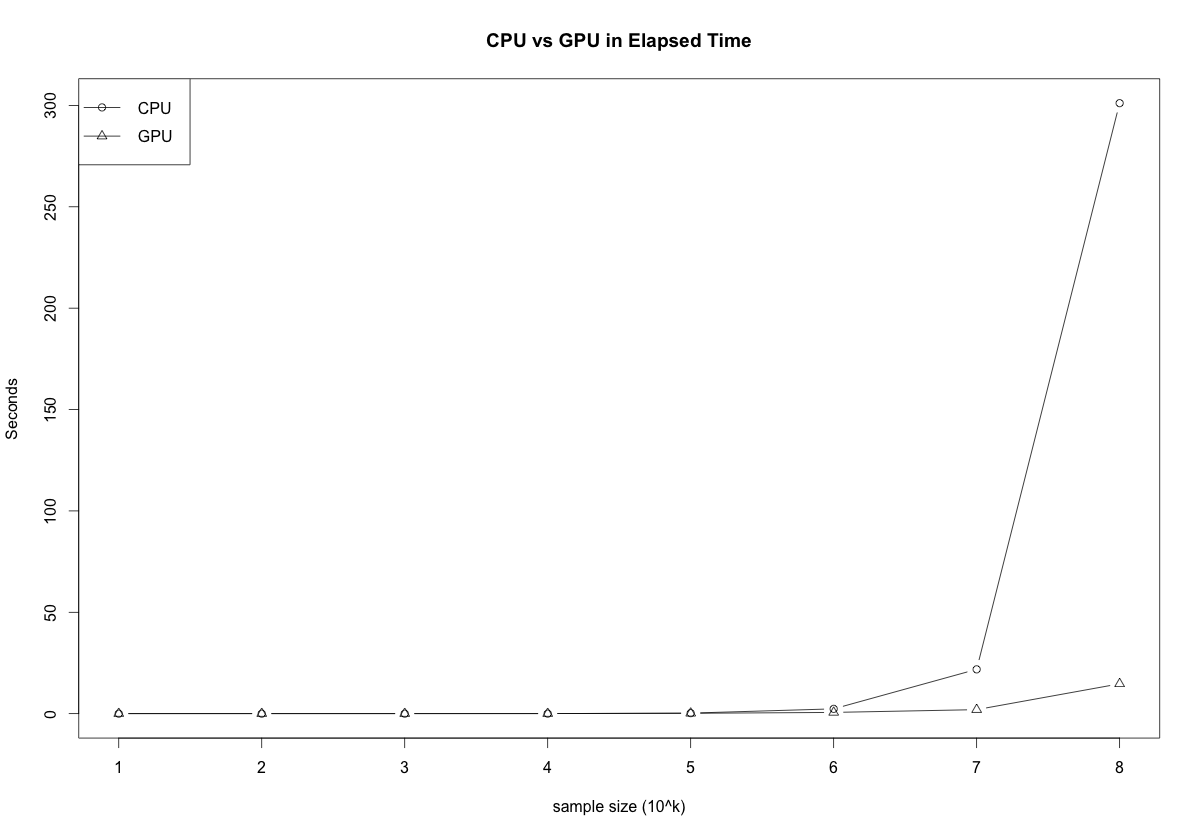
\includegraphics[width=\textwidth]{cpuvsgpuet.png}\newline
Apparently when sample sizes are small ($k = 1, \cdots, 6$), GPU did not offer much difference from CPU; however, when sample size got large ($k = 7, 8$), the time needed for CPU to complete each task grew exponentially, whereas GPU only required moderately more time than smaller sample sizes. Also most of the time increased for GPU was the "User Time", namely time needed transferring data between host and device.\newline
For verification purposes, both CUDA and R codes were tested with three different truncated normal distributions: $TN(2, 1; -\infty, 0), TN(2, 1; 0, \infty), \newline TN(0, 1; -\infty, -10)$. 10000 samples were generated with GPU and CPU respectively, and the means are listed below together with expected values:
\begin{center}
	\begin{tabular}{|c|c|c|c|}
	\hline
	Distribution & $E(Z)$ & GPU & CPU \\
	\hline
	$TN(2, 1; -\infty, 0)$ & -0.373 & -0.374 & -0.374 \\
	\hline
	$TN(2, 1; 0, \infty)$ & 2.055 & 2.057 & 2.057 \\
	\hline
	$TN(0, 1; -\infty, -10)$ & -10.098 & -10.098 & -10.098 \\
	\hline	
	\end{tabular}
\end{center}
The results in the table above showed that both my GPU and CPU code works for one-sided truncated normal distributions as well as in the tail region.
\newline \newline
Problem 2 \newline \newline
In this problem, we implemented Gibbs sampler algorithm for Probit MCMC, whose model is given by
\begin{align*}
	Y_i|Z_i &\sim \mathbf{1}_{\{Z_i > 0\}} \\
	Z_i | \beta &\sim N(x^T_i\beta, 1) \\
	\beta &\sim N(\beta_0, \Sigma_0)
\end{align*}
Firstly we need to set up the Gibbs sampler by finding marginal posterior distributions of $Z_i^{(t+1)}|Y_i, \beta^{(t)}$ and $\beta^{(t+1)}|Z_1^{(t+1)},\cdots, Z_n^{(t+1)}$, i.e. in each iteration of Gibbs sampler, we want to sample $Z_i$'s first, then update $Z_i$ to sample $\beta$. For $Z_i^{(t+1)}$ from the lecture note, we have
\begin{align*}
	Z_i^{(t+1)}|Y_i, \beta^{(t)} \sim \begin{cases}
		TN(x_i^T\beta^{(t)}, 1; -\infty, 0) &\mbox{when } Y_i = 0 \\
		TN(x_i^T\beta^{(t)}, 1; 0, \infty) &\mbox{when } Y_i = 1 \\
	\end{cases}
\end{align*}
Next we need to obtain the marginal posterior distribution for $\beta^{(t+1)}|Z_1^{(t+1)},\cdots, Z_n^{(t+1)}$. Let $X = (x_1^T,\cdots,x_n^T)^T, Z = (Z_1, \cdots, Z_n)^T$, then we can see that $Z|\beta \sim N(X\beta, \mathbf{I})$. So for the marginal posterior distribution of $\beta$, we have
\begin{align*}
	p(\beta|Z) &\propto p(\beta)p(Z|\beta) \\
	&\propto exp\{-\frac{1}{2}[(Z - X\beta)^T(Z-X\beta) + (\beta - \beta_0)^T\Sigma_0^{-1}(\beta - \beta_0)]\} \\
	&\propto exp\{-\frac{1}{2}(\beta^TX^TX\beta - 2Z^TX\beta + \beta^T\Sigma_0^{-1}\beta -2\beta_0^T\Sigma_0^{-1}\beta)\}
\end{align*}
By Bayesian theory, given the facts that $\beta$ has a normal prior distribution and the distribution of $Z|\beta$ is also normal, the posterior distribution for $\beta$ should also be normal, more precisely multivariate normal distribution. We can extract the parameters of that normal distribution from the above quadratic expression  of $\beta$:
\begin{align*}
	&\beta^TX^TX\beta - 2Z^TX\beta + \beta^T\Sigma_0^{-1}\beta -2\beta_0^T\Sigma_0^{-1}\beta \\
	&= \beta^T(X^TX + \Sigma_0^{-1})\beta -2(Z^TX+\beta_0^T\Sigma_0^{-1})\beta
\end{align*}
If $\beta \sim N(\mu_\beta, \Sigma_\beta)$, then the quadratic expression would contain the following terms:
\begin{align*}
	\beta^T\Sigma_\beta^{-1}\beta -2\mu_\beta^T\Sigma_\beta^{-1}\beta
\end{align*}
Matching corresponding terms in the expression, we get
\begin{align*}
	\Sigma_\beta^{-1} &= (X^TX+\Sigma_0^{-1}) \\
	\Rightarrow \Sigma_\beta &= (X^TX+\Sigma_0^{-1})^{-1} \\
	\mu_\beta^T\Sigma_\beta^{-1} &= (Z^TX+\beta_0^T\Sigma_0^{-1}) \\
	\Rightarrow \Sigma_\beta^{-1}\mu_\beta &= (Z^TX+\beta_0^T\Sigma_0^{-1})^T \\
	&= (\Sigma_0^{-1}\beta_0 + X^TZ) \\
	\Rightarrow \mu_\beta &= \Sigma_\beta\Sigma_\beta^{-1}\mu_\beta \\
	&=(X^TX+\Sigma_0^{-1})^{-1}(\Sigma_0^{-1}\beta_0 + X^TZ)
\end{align*}
Therefore we obtain the second step in Gibbs sampler: sample $\beta^{(t+1)}|Z^{(t+1)}$ from multivariate normal distribution
\begin{center}
	$N[(X^TX+\Sigma_0^{-1})^{-1}(\Sigma_0^{-1}\beta_0 + X^TZ^{(t+1)}), (X^TX+\Sigma_0^{-1})^{-1}]$
\end{center} 
Overall the Gibbs sampler generally goes:
\begin{enumerate}[(1)]
	\item Initialize by setting $\beta_0, \Sigma_0$ and $t= 0$.
	\item Obtain the vector $Z^{(t+1)}$ by sampling each $Z_i^{(t+1)}$ from corresponding truncated normal distribution, either $TN(x_i^T\beta^{(t)}, 1; -\infty, 0)$ when $Y_i = 0$ or $TN(x_i^T\beta^{(t)}, 1; 0, \infty)$ when $Y_i = 1$.
	\item Sample $\beta^{(t+1)}$ from the multivariate normal distribution given above.
	\item Check for convergence, if not, increment $t$ to $t+1$, go to step (2) and iterate.
\end{enumerate}
In our case, we set $\beta_0 = \mathbf{0}, \Sigma_0 = \mathbf{I}$. Since the homework mainly focused on comparing CPU and GPU performances, the convergence of generated Markov chain was not tested.
For the CPU code, I programmed the algorithm in R. For the GPU code, the only part completed on GPU was sampling $Z^{(t+1)}$ by using .cuda() to call the kernel function coded in problem 1, and the rest goes very similarly to CPU code in R. With provided R script, five datasets was simulated; however only the first four datasets were used, because the last one was quite large and not feasible to compute within reasonable time. Additionally only $600$ iterations were executed for each dataset with the first $100$ deemed as "burnin" iterations. 


\end{document}
